\CHAPTER{DC readout - evaluation}
\label{chapter5}
%\doublespace

\SECTION{Sensitivity}

The primary figure of merit of a gravitational wave detector is its
noise floor, calibrated as a strain spectral density.  When evaluating
DC readout in Enhanced LIGO, we can begin by looking at the noise
floor: was the promised sensitivity delivered?  For the readout, the
answer is a resounding yes.  Given the input power and other known
parameters of the interferometer, the noise floor is accurately
modeled.

\SUBSECTION{Shot noise limited sensitivity}

The predicted curve is produced by dividing the shot noise level
(spectral density $\sqrt{h (c/\lambda) P_AS}$ by the optical gain

$$\sqrt{2 P_{IN} P_{AS}} g_{cr} r_{cp}
\left(\frac{2\pi}{\lambda}\right) \left| \frac{1}{1 +
  i\frac{f}{f_c}}\right|$$ while accounting for the various
inefficiencies in the system (listed in table XX).

The Hanford detector was able to operate at a much higher input power,
and has a better power recycling gain than the Livingston detector.
However, mode-matching of the OMC to the arm cavity mode was only
$\sim70\%$, limiting the performance.

\begin{figure}
\subfloat[Hanford][Hanford]{
  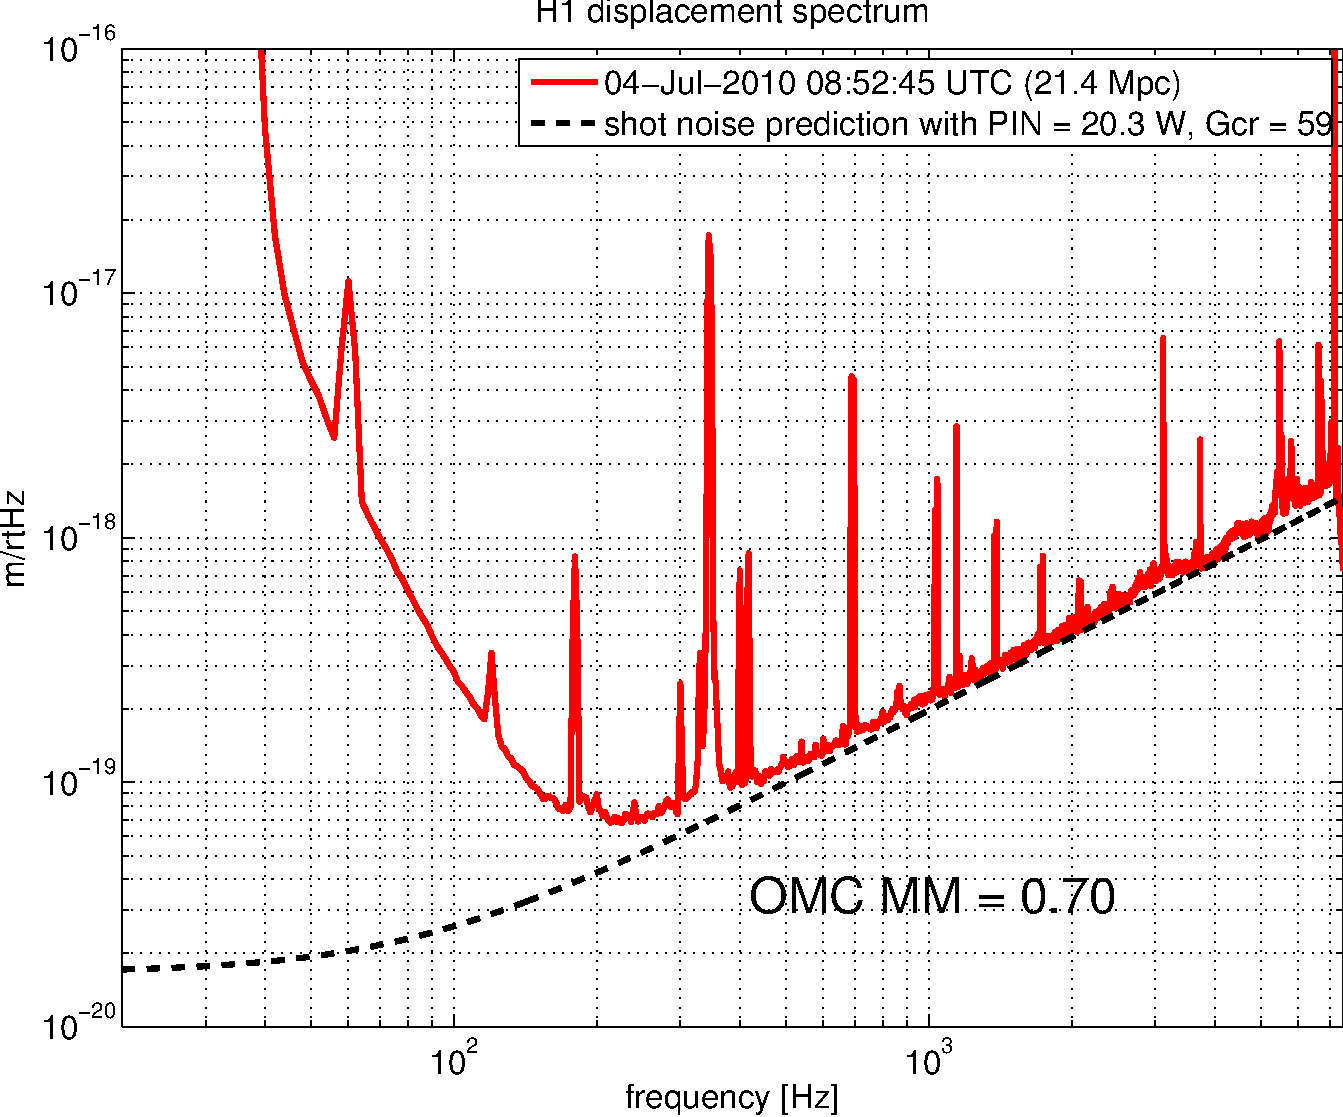
\includegraphics[width=0.48\columnwidth]{chapter5/figures/H1-962268780.pdf}
}
\subfloat[Livingston][Livingston]{
  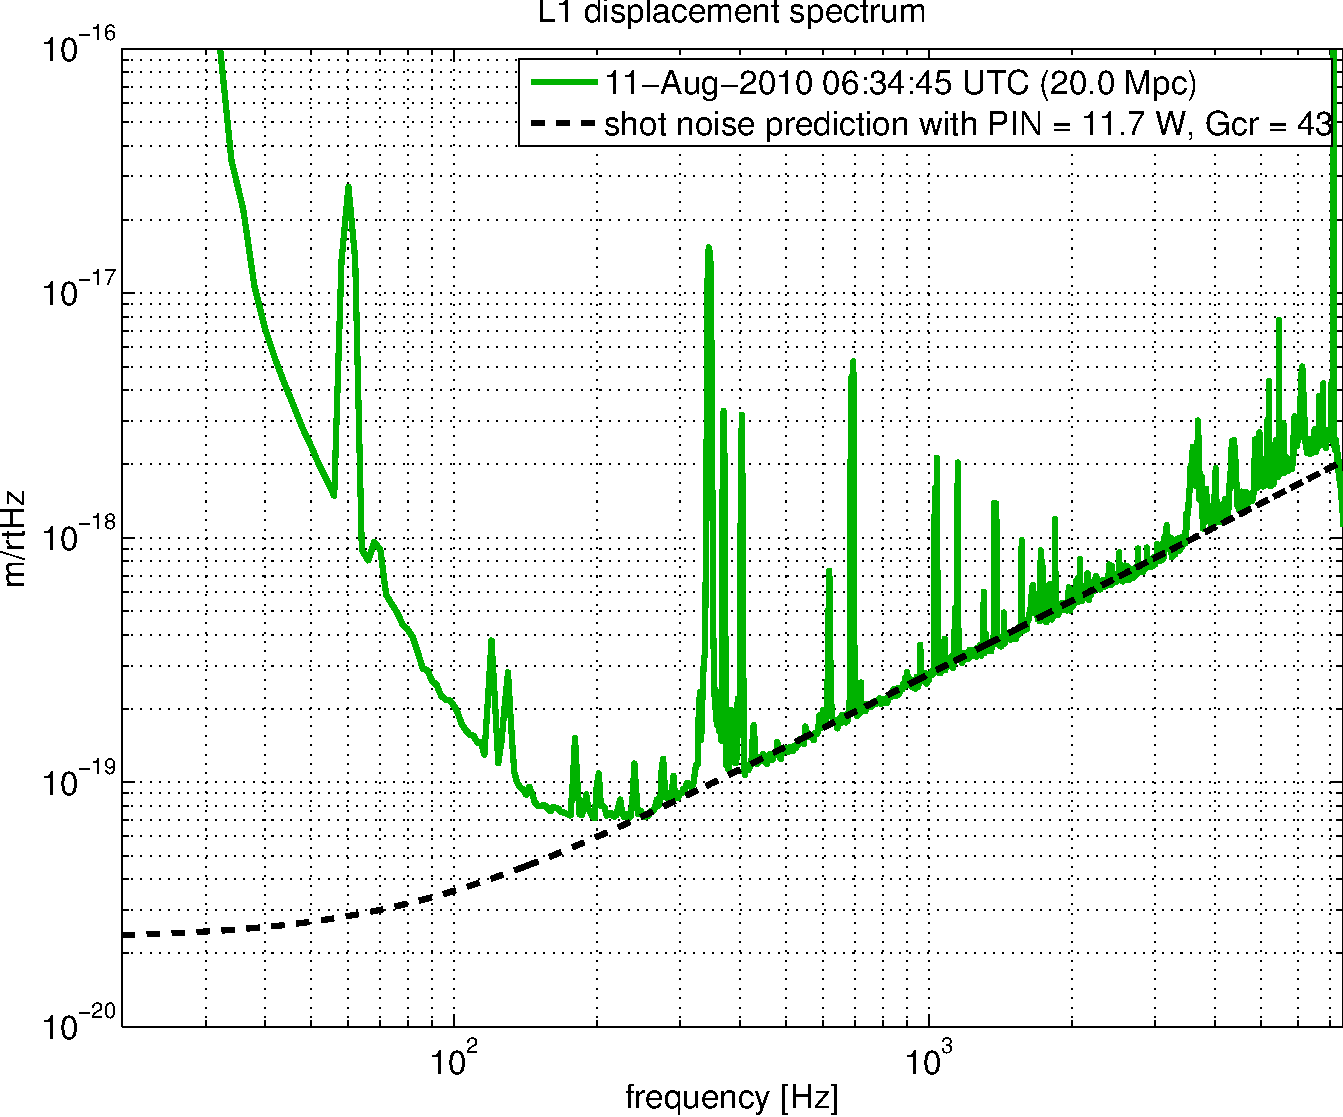
\includegraphics[width=0.48\columnwidth]{chapter5/figures/L1-965543700.pdf}
}
\caption{\label{fig:shot-noise-limited-sensitivity}Shot noise limited sensitivity of the Livingston and Hanford detectors.}
\end{figure}



%% Cavity properties [Table]
% These values are all from Sam's document T080144:
% https://dcc.ligo.org/cgi-bin/private/DocDB/ShowDocument?docid=5416
\begin{table}
\centering
\begin{tabular}{l l l l l}
\hline 
\textbf{parameter}          &\textbf{Hanford}&\textbf{Livingston}  \\
\hline
arm cavity phase gain       & 137            & 137         \\
input optics efficiency     & 0.82           & 0.75        \\
interferometer mode-matching&                & 0.92        \\
carrier recycling gain      & $59\pm6$       & 41          \\
modulation depth            & 0.34           & 0.33        \\
OMC transmission            & 0.97           &             \\
OMC mode-matching           & 0.70           & 0.95        \\
Output Faraday transmission & $0.94\pm0.02$  & 0.9805      \\
DC-readout path pickoff     & 0.953          & 0.972       \\
PD quantum efficiency       & 0.98           &             \\
\hline
\end{tabular}
\caption{Designed and measured properties of the Hanford and Livingston interferometers.}
\label{tab:IFOproperties}
\end{table}


\SECTION{Laser and Oscillator noise couplings}

The coupling of noises from the laser source and RF oscillators to the
gravitational wave readout channel differ considerably in RF and DC
readouts.  In addition, DC readout with an OMC is generally much more
sensitive to beam motion (jitter).  These couplings are of primary
interest in designing the optical readout of a gravitational wave
detector.

\SUBSECTION{Laser noises}

\begin{figure*}[]
% Laser AM
\subfloat[Laser amplitude noise coupling (L1)][Laser amplitude noise coupling (L1)]{
  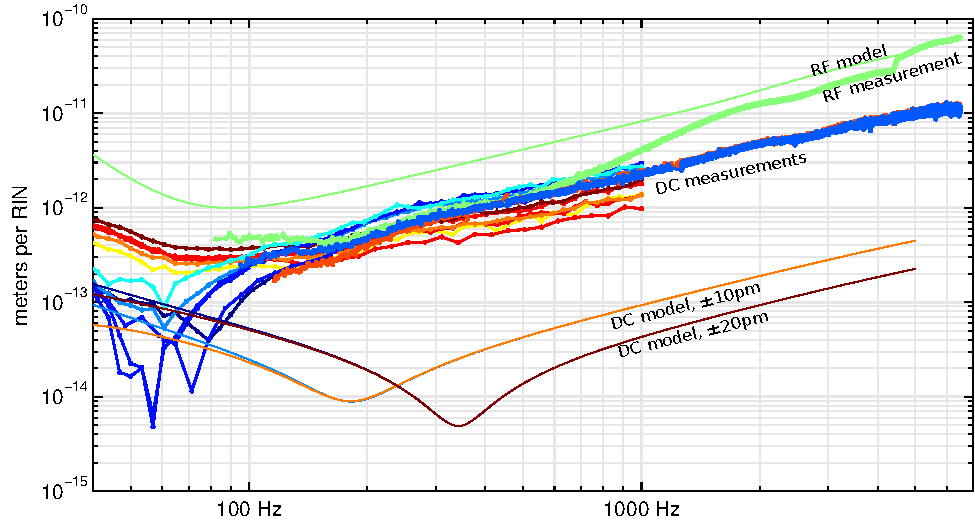
\includegraphics[]{figures/laserAM-L1.pdf}
  \label{fig:laser-AM}
}
\subfloat[Laser amplitude noise coupling (H1)][Laser amplitude noise coupling (H1)]{
  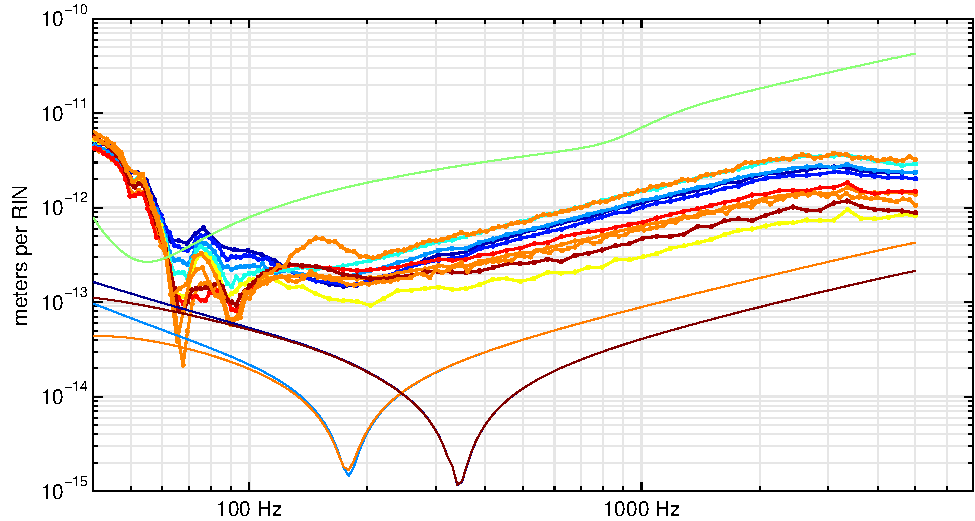
\includegraphics[]{figures/laserAM-H1.pdf}
  \label{fig:laser-AM-H1}
}

% Laser FM
\subfloat[Laser frequency noise coupling (L1)][Laser frequency noise coupling (L1)]{
  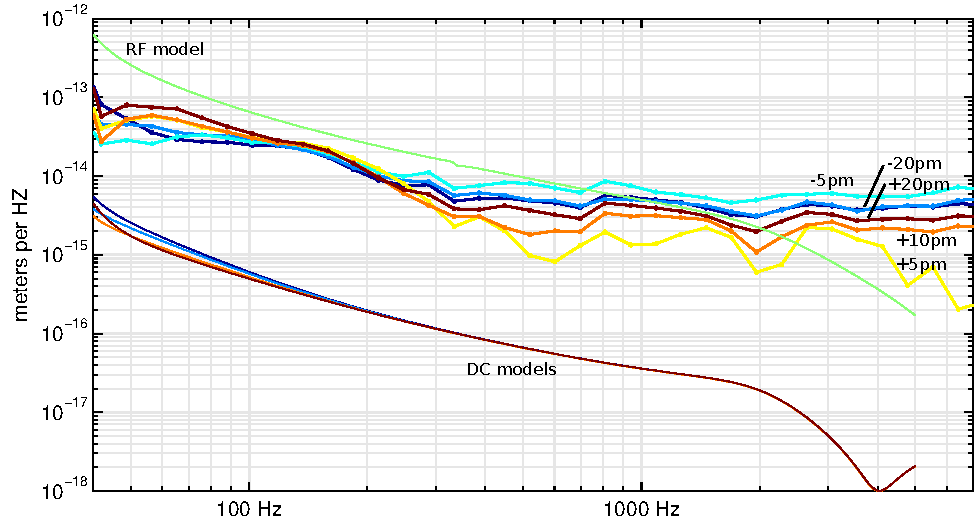
\includegraphics[]{figures/laserFM-L1.pdf}
  \label{fig:laser-FM}
}
\subfloat[Laser frequency noise coupling (H1)][Laser frequency noise coupling (H1)]{
  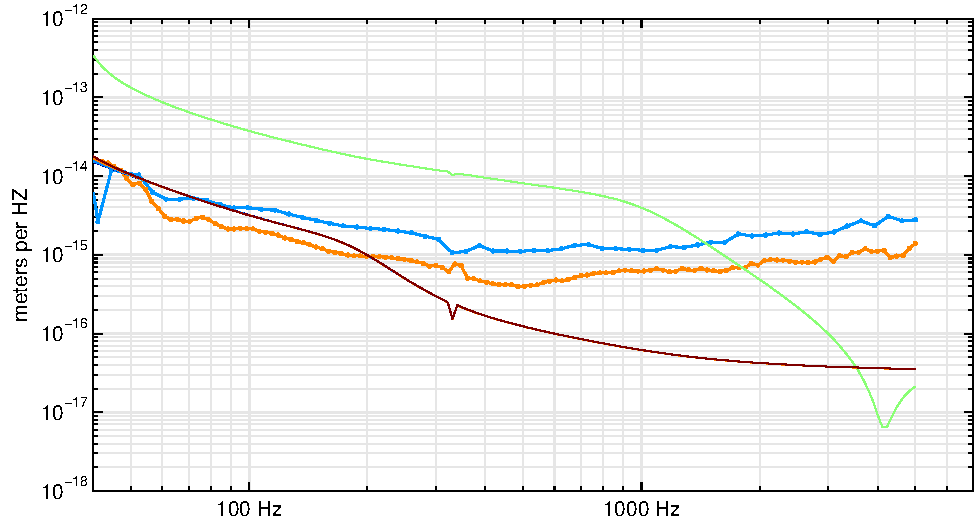
\includegraphics[]{figures/laserFM-H1.pdf}
  \label{fig:laser-FM-H1}
}
\end{figure*}


\SUBSECTION{Oscillator noises}
%
Reduced coupling of noises from the RF oscillator is one of the motivations
for implementing DC readout. Despite not relying on the sidebands
directly, behavior of the RF oscillator is still able to sneak into
the DC readout. 

\begin{figure*}
% Oscillator AM
\subfloat[Oscillator amplitude noise coupling (L1)][Oscillator amplitude noise coupling (L1)]{
  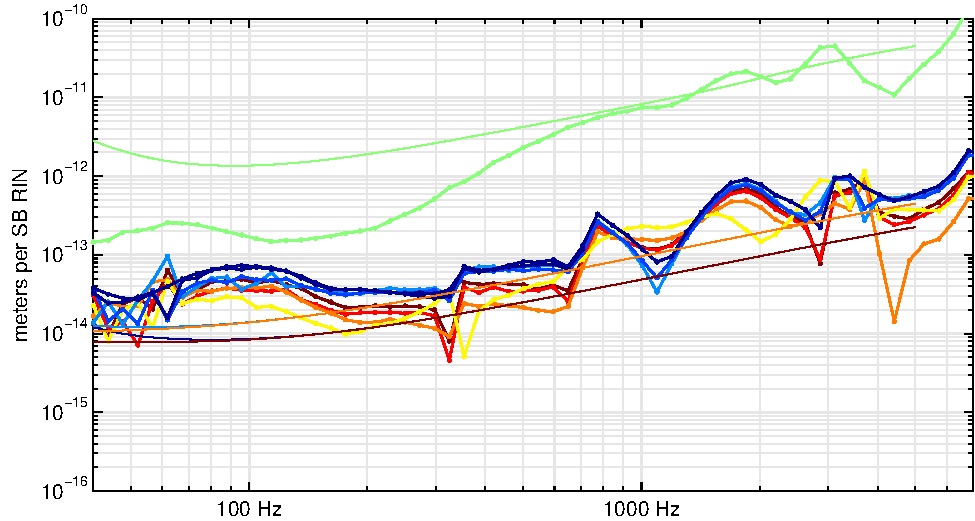
\includegraphics[]{figures/oscAM-L1.pdf}
  \label{fig:osc-AM}
}
\subfloat[Oscillator amplitude noise coupling (H1)][Oscillator amplitude noise coupling (H1)]{
  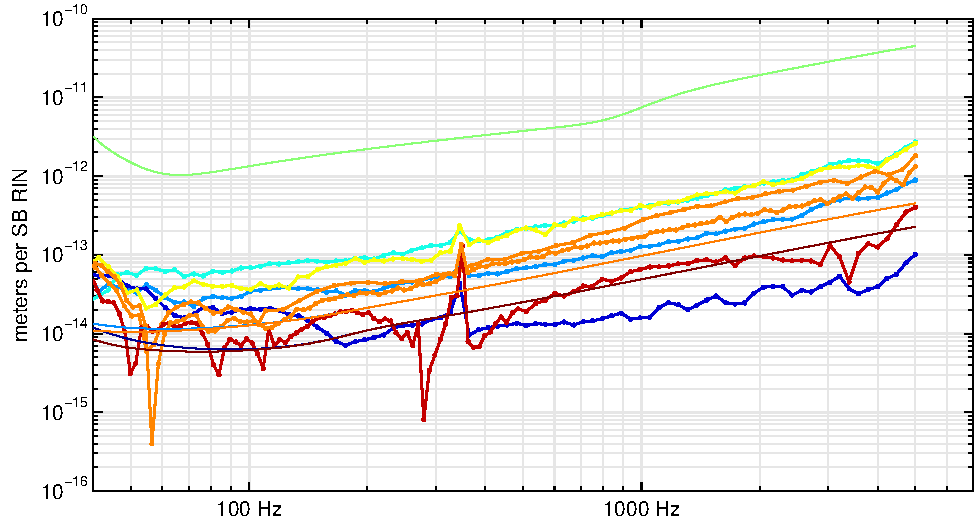
\includegraphics[]{figures/oscAM-H1.pdf}
  \label{fig:osc-AM-H1}
}

% Oscillator PM
\subfloat[Oscillator phase noise coupling (L1)][Oscillator phase noise coupling (L1)]{
  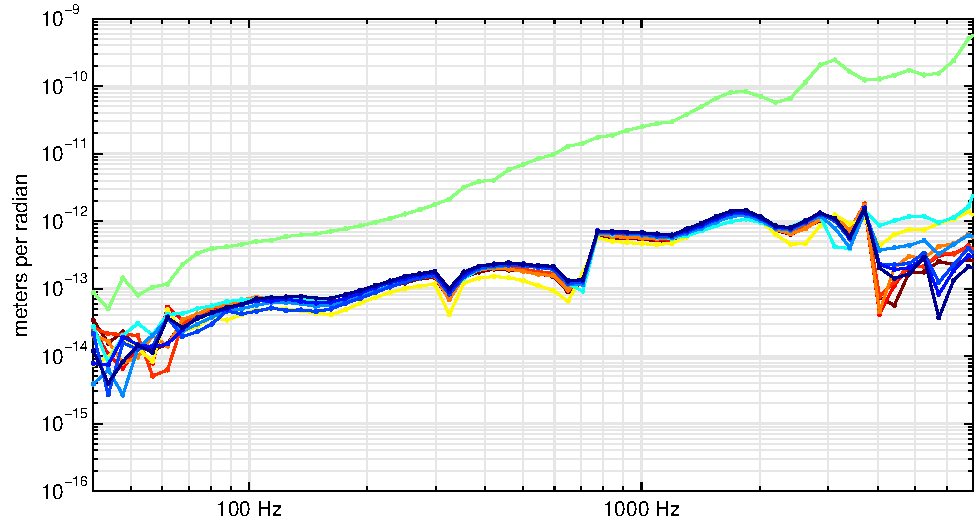
\includegraphics[]{figures/oscPM-L1.pdf}
  \label{fig:osc-PM}
}
\subfloat[Oscillator phase noise coupling (H1)][Oscillator phase noise coupling (H1)]{
  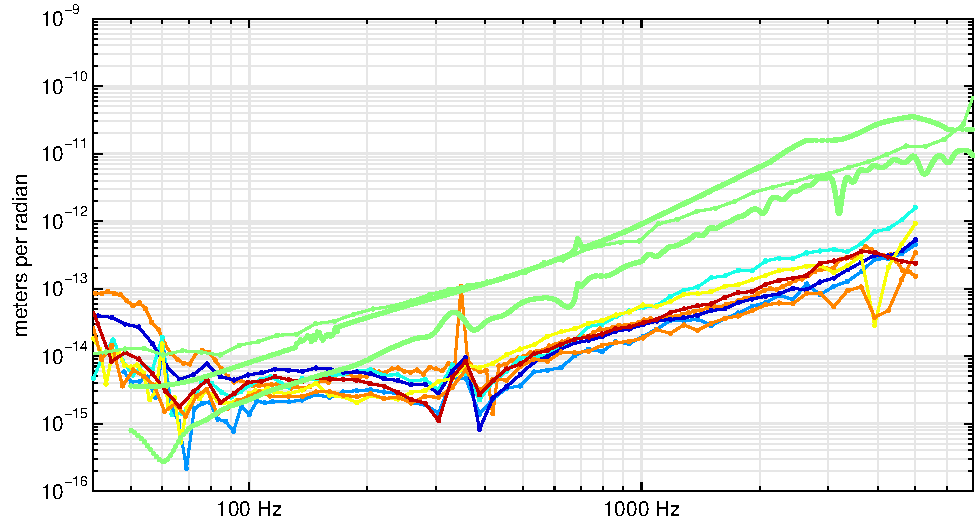
\includegraphics[]{figures/oscPM-H1.pdf}
  \label{fig:osc-PM-H1}
}

\caption{\label{noise-couplings}Oscillator and laser noise couplings to the gravitational wave readout channel, calibrated in equivalent displacement (meters).  Solid lines are the results of a frequency-domain, plane-wave model; dotted lines are linear transfer function measurements.  Color represents the DARM offset, with warm colors for positive offsets and cool colors for negative offsets.  Measurements and models for RF readout are in green.}
\end{figure*}

One coupling path is conversion of Oscillator AM to laser intensity
AM via the RF modulator. The sideband RIN per oscillator AM is given
by \[
2\Gamma_{0}\frac{J_{1}'(\Gamma_{0})}{J_{1}(\Gamma_{0})}=\Gamma_{0}\frac{J_{0}-J_{2}}{J_{1}}\]
(see Livingston elog 2010-07-15, {}``sideband RIN per oscillator
AM calculation,'' ).

Measured coupling is shown in figure \ref{fig:oscillator-AM-coupling-measured}.



\SUBSECTION{Oscillator phase noise}
%
Oscillator phase noise sneaks in via some dirt effect. Look at how
much better it is in DC readout!

Measured coupling of oscillator phase noise to the readout channel
is shown in figure \ref{fig:oscillator-PM-coupling-measured}.

\SECTION{Beam jitter noise}
%
Beam jitter noise is perhaps the most important new noise source in
DC readout and is tied to alignment of the OMC, which has proved to
be one of the most subtle new issues. The output mode cleaner converts
motion of the input beam into variations in transmission. The resulting
variation in the transmitted light level is indistinguishable from
DARM motion.

\SECTION{Electronics noise}
%
The DC readout system provides a quantum-limited readout at $\sim100$
Hz. Careful engineering ensures that we are not limited by electronics
thermal noise or $1/f$ flicker noise.

\SECTION{Optical spring}
%
Detuning the arm cavities from their resonance introduces a big optical
spring. This doesn't seem to have any measurable effect.

\SECTION{Nonlinearity  of the DC error signal}
%
Although we operate sufficiently far from the dark fringe that the
linear coupling of residual DARM motion to output power is dominant,
sufficiently large motion could produce second-order coupling. Fortunately,
this turns out to be totally negligible.

\SECTION{Noise budget}
\SECTION{Optical gain}

\SECTION{Digital effects}

The realtime digital signal processing system through which our
control systems are implemented provide the illusion of a continuous,
analog system.  However, it is important to remember that the
underlying system operates on quantized values in discrete time in
order to avoid being caught by surprise by ``digital noises''.

1. Finite, non-deterministic execution time
2. ADC bit noise
3. Floating point dynamic range
4. Synchronized communications
